%Over the course of this report we have refered to, and approximated, the distribution of variouss classifications of prime numbers. Using now our implementation of Helfgott's origianl code we seek to present the legitimacy of said distributions and also reflect on the quality of the code which we have written. The specific distributions to be presented are those of the regular prime numbers, the twin primes, and a the frequency of various prime gaps will also be presented. For each of these implementations have slight modifications been made to the code, which will be briefly discussed.

Genom rapportens gång har vi hänvisat till, och uppskattat fördelningen av, ett antal klasser av primtal och deras egenskaper. 
Nu kommer vi att redovisa några resultat som ovan nämnda Python-program givit.
Vi börjar med att räkna primtal i ett intervall och jämföra det med primtalssatsen, detta i syftet att övertyga oss om kodens validitet. 
Sedan undersöker vi trovärdigheten hos en förmodad fördelning för mängden av primtalstvillingar. 
Slutligen redovisas frekvensen av primtalsgap, och mönster som uppstår från detta.

\subsubsection{Fördelningen av primtal}\label{app.primes.title}
%Beginning with the classic example of the set of prime numbers, below is illustrated the distribution predicted by the familiar x over log x from sieve theory/Chebychev, the more accurate lorgarithmic integral Li(x), and the actual number of primes found in using our implementation. In order to generate the following graph, no new sieving methods were introduced, simply the counting fucntion in Appendix X

Vi börjar med att jämföra antalet primtal som hittats med \textsc{NewSegSiev}, mot fördelningen som ges av primtalssatsen, nämligen
\begin{equation}
    \pi(x) \sim \text{Li}(x) = \int_2^x\frac{1}{\log t}dt\label{app.primes.PNT}.
\end{equation}
För att skapa figur \ref{fig:res.prime} använder vi vår implementering av Helfgotts kod och en enkel räknefunktion.

\begin{figure}[h] %[H]
    \centering
    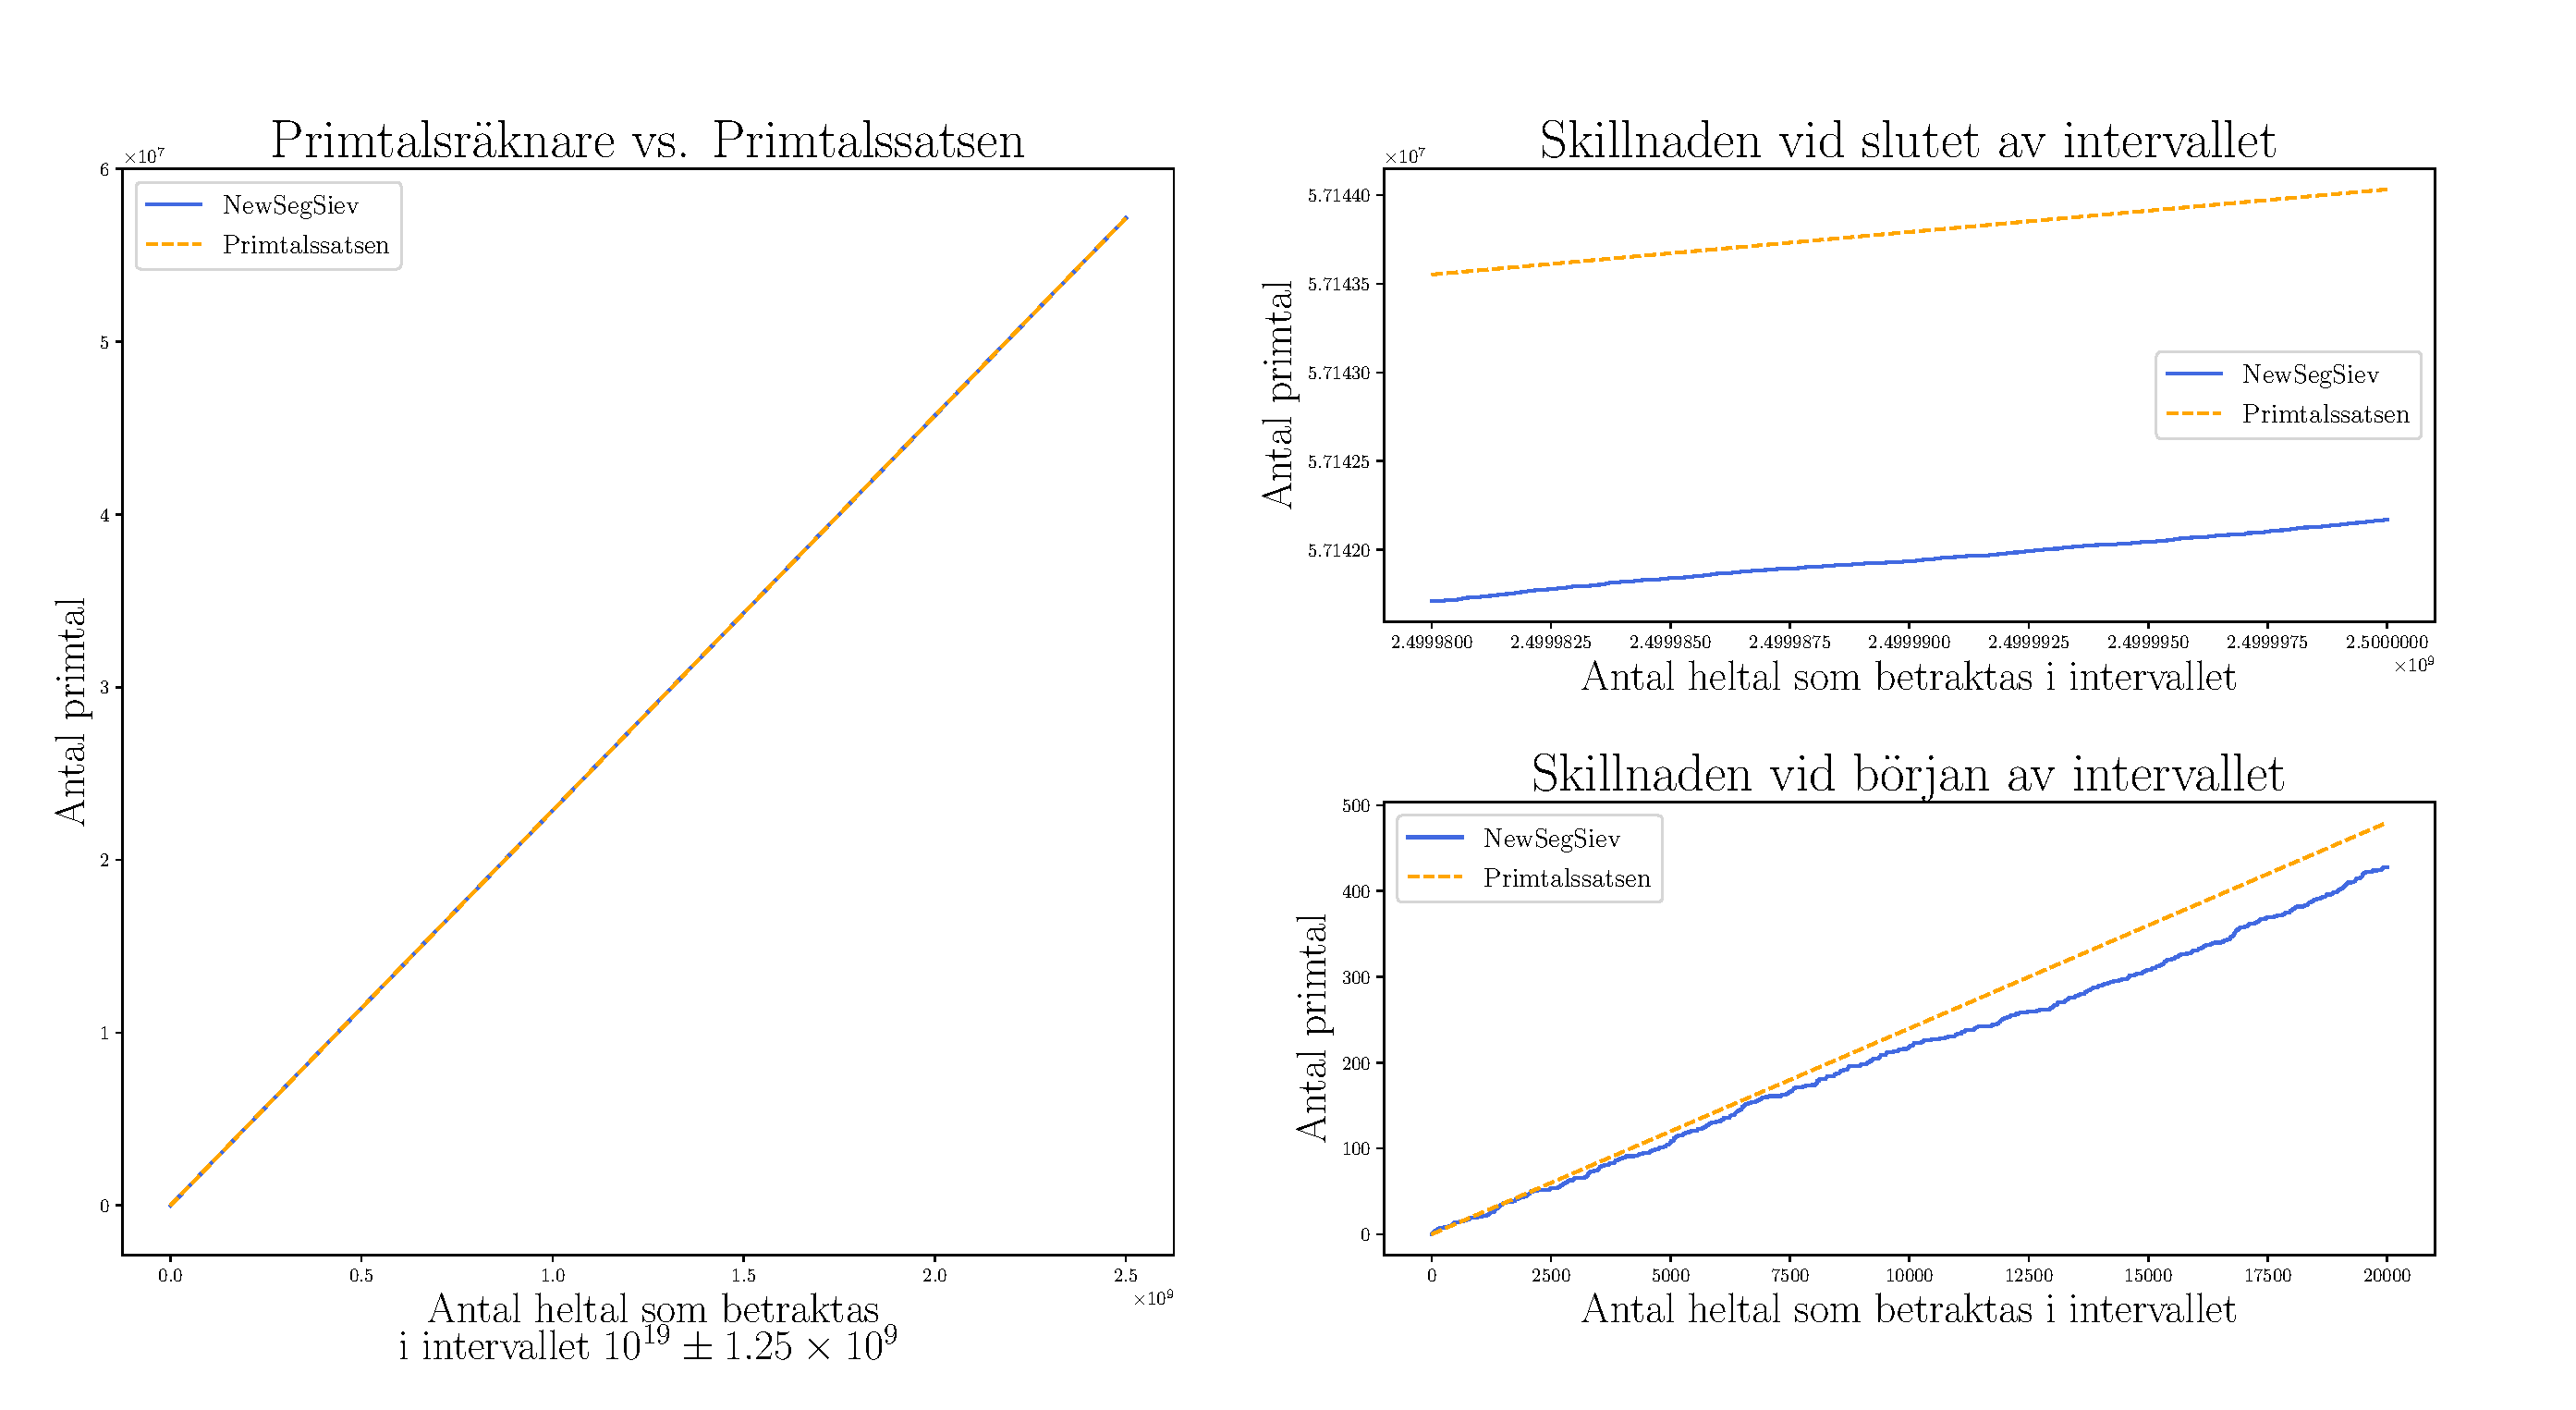
\includegraphics[width = \textwidth]{coen/Images/Primes.pdf}
    \caption{I figuren till vänster redovisas antalet primtal som förväntas enligt primtalssatsen, \textit{orange}, och antalet primtal som hittades enligt \textsc{NewSegSiev}, \textit{blå}, då \(n = 10^{19}\), \(\Delta = 1.25\cdot10^{9}\), och \(K = 2.5\). 
    Notera att kurvorna ligger nästan på varandra. 
    I grafen till höger redovisas inzoomade versioner av grafen till vänster för att visa skillnaden mellan vår mätning och det som förväntas vid början av intervallet, där algoritmen returnerar kring 100 färre primtal än förväntat, och vid slutet av intervallet, där algoritmen returnerar kring 2000 färre.
    Dock att kurvorna inte ligger på varandra är väntat eftersom det finns ett fel i \ref{app.primes.PNT} vilket inte visas.}
    %This graph shows the relative distributions of primees as per the aforementioned fucntions. Notice that while x over log x appears relatively close for smaller x the logarithmic integral approximation is a near exact match for the true distribution, so much so that the code line is hidden.
    \label{fig:res.prime}
\end{figure}
%As shown in figure X, should we believe in the PNT it seems as though our code does indeed find the correct number of primes. The rather large error in the x over log x estimate is indicative/reflective of one of the limitations highlighted in Section XXX, namely the impact of the error terms and their reconcillation with the main terms. Howeve, there doest exist a deeper link between the x over log x estimate and that of the logarithmic integral. Throguh the use of integral wizardry you can decompose the logarithmic integral into a series of terms, the first of which being x over log x with the remainder being of the order of sqrt(x). This then accounts for the increase in error as x grows. Thiese kinds of approximations for the prime counting function can also be rather naturally extrapolated to those for twin primes, as discussed below.

Som vi ser i vänstra grafen av figur \ref{fig:res.prime} är skillnaden mellan kurvorna nästan osynlig på makronivå, och eftersom primtalssatsen gäller är det troligt att vårt program har hittat det korrekta antalet primtal i intervallet.
Att de inte ligger exakt på varandra är huvudsakligen beroende på felet vilket inte visas i \eqref{app.primes.PNT}.
Notera att vi normaliserar felet vid början av intervallet eftersom vi betraktar skillnaden \(\text{Li}(x) - \text{Li}(n - \Delta)\), \(x\in[n-\Delta,\; n+\Delta]\).
Att vår kod hittar ungefär 100 färre primtal än förväntat efter 20 000 heltal och ungefär 2000 färre primtal efter \(2.5\times10^9\) heltal är mycket rimligt då felet i \eqref{app.primes.PNT} kan som bäst vara \(O(2\Delta)^{1/2 + \varepsilon}),\; \varepsilon > 0\), under antagandet att Riemannhypotesen stämmer \cite[kap. 5]{RiemannErr}.

Värdet på \textit{n} valdes till \(10^{19}\) för att detta är stort nog för att vara intressant men inte så stort att programmets körningstid blir orimlig\footnote{Att \textit{n} inte valdes större i detta fallet är på grund av körningstiden för koden.}.
Vi valde \(\Delta\) till \(1.25\times10^9\) får att nyttja de tidbesparingar som fås av att gå in i den andra loopen i \textsc{NewSegSiev}.
Slutligen valde  vi \textit{K} till 2.5 för att det är minsta möjliga värde per konstruktion av algoritmen.
Vi kommer nu att studera den data som programmet gav efter körning med ovanstående parametervärden.

\subsubsection{Fördelningen av primtalstvillingar}
%Continuing our presentation of various sets of prime's distributions, next we turn to the other recurring theme of twin primes. The following figure illustrates the distributions of twin primes as predicted by x over log squared x and the second order logarithmic integral against those primes found using our implementation. It should be noted that a rather simple help function, Appendix XXX, was written which searches for non twin primes in the prime list and removes them.

Med hjälp av de primtal vi hittade i \ref{app.primes.title}, vänder vi oss nu till primtalstvillingar. Det finns ingen sats för primtalstvillingar motsvarande primtalssatsen, dock så finns det en förmodan framlagd av Hardy och Littlewood \cite[Förmodan B]{Hardy}. 
Den lyder
\begin{equation}
    \pi_2(x) \sim 2\text{C}_2\cdot \text{Li}_2(x) = 2\text{C}_2\int_2^x\frac{1}{(\log t)^2}dt\label{app.twins.TWN}
\end{equation}
där \(\text{C}_2 = 0.66016...\) är primtalstvillingskonstanten \cite{TwinPrimeConstant}. Jämför vi den hypotetiska fördelningen emot antalet primtalstvillingar vi har genererat, så får vi figur \ref{fig:res.twins}.

\begin{figure}[h]
    \centering
    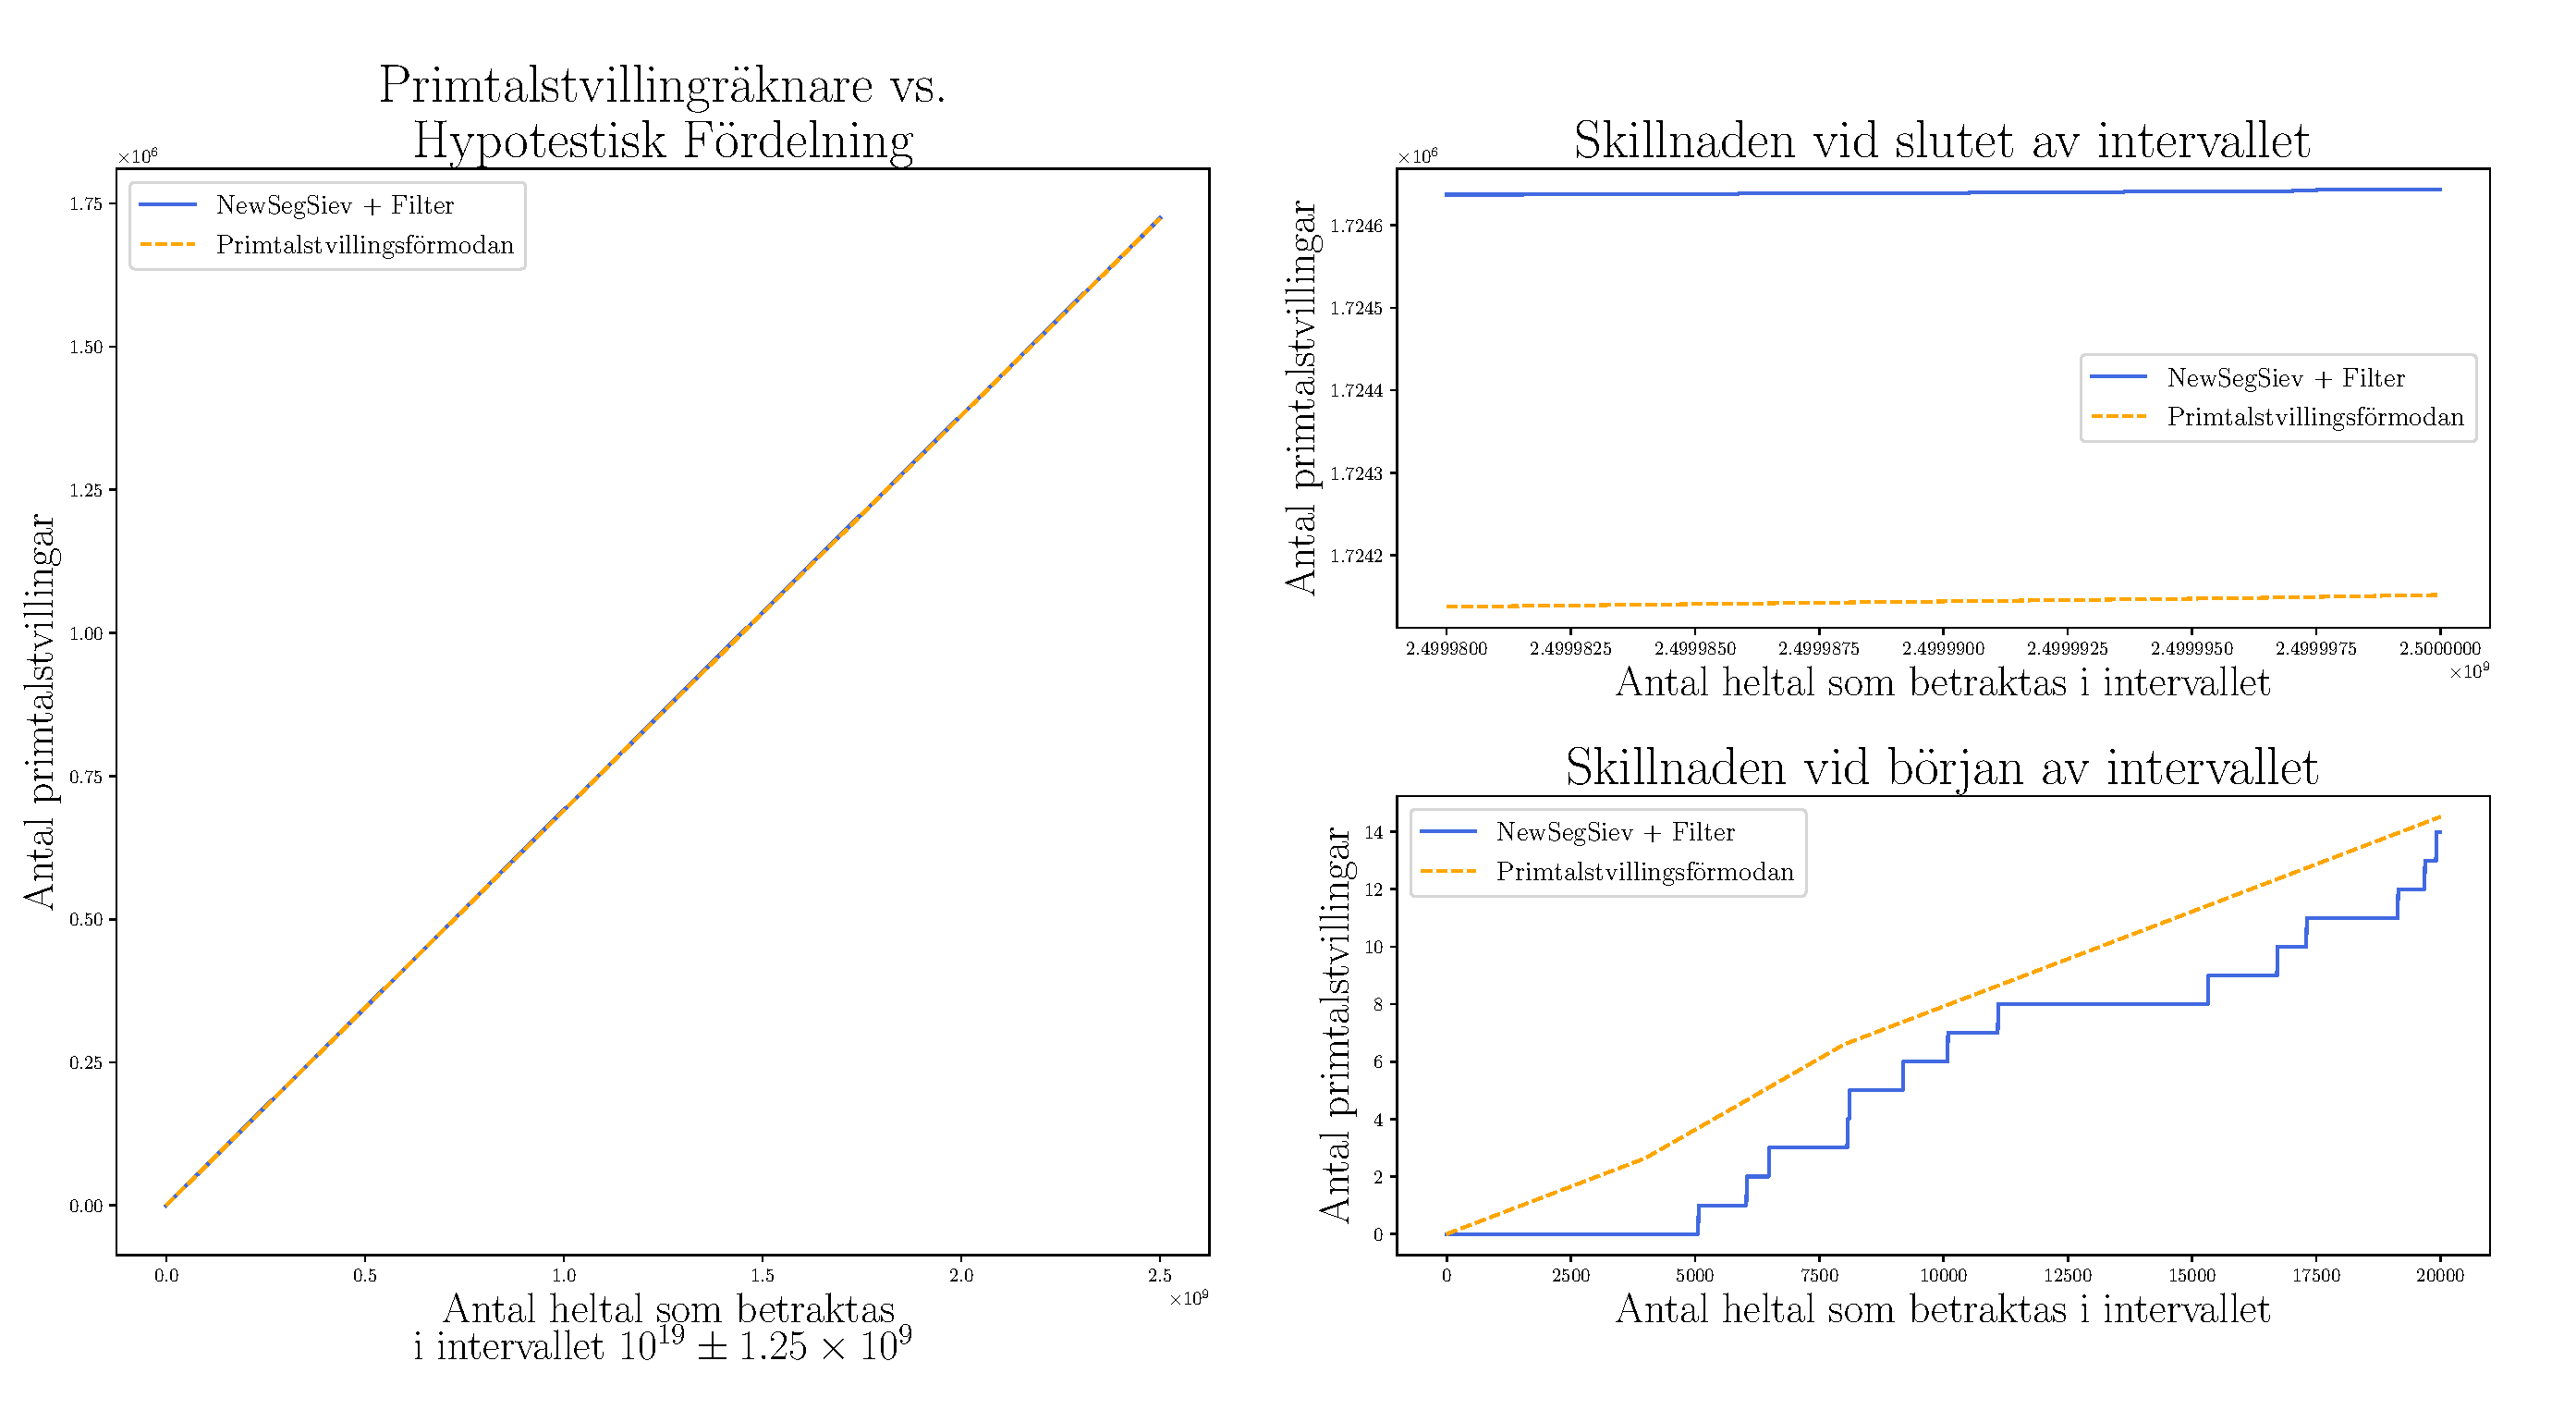
\includegraphics[width = \textwidth]{coen/Images/TwinPrimesNoKapp.pdf}
    \caption{I grafen till vänster redovisas antalet primtalstvillingar som förväntas enligt den hypotetiska fördelningen, \textit{orange}, och de primtalstvillingar som hittades enligt \textsc{NewSegSiev}, \textit{blå}, då \(n = 10^{19}\), \(\Delta = 1.25\times10^9\), och \(\text{C}_2\) har avrundats till 0.66. Notera återigen att kurvorna ligger nästan på varandra. I graferna till höger så redovisas inzoomade versioner av grafen till vänster. 
    Översta grafen till höger visar skillnaden mellan antalet primtalstvilling vi har hittat och antalet som förväntas vid slutet av intervallet, där algoritmen returnerar 500 fler primtalstvillingar. Efter de första 20 000 heltalen i intervallet så har algoritmen genererat nästan det exakta antalet primtalstvillingar som förväntas.}
    %This graph shows the relative distributions of the twin primes as per the aforementioned fucntions. Notice once again the accuarcy of the logarithmic integral, once again hiding our code line, as opposed to that of C x over log squared x, where the constant is 2*C_2, or 2 times the twin prime constant (discussed below).
    \label{fig:res.twins}
\end{figure}

Datan i figur \ref{fig:res.twins} ger oss några intressanta insikter angående primtalstvillingar. 
Den första är att datan ger stöd till den hypotetiska fördelningen av primtalstvillingar. 
Kurvorna ligger mycket nära varandra och stödjer därmed hypotes \ref{app.twins.TWN}, eftersom vi nu litar på vårt program.
Skillnaden mellan det förväntade antalet primtalstvillingar och antalet som hittades är som mest ungefär 500, och hittas vid slutet av intervallet.
I sammanhanget av ett intervall av längd \(2.5\times10^9\) så är en skillnad av 500 ekvivalent med en avvikelse av \(2\times 10^{-7}\) mer primtalstvillingar per heltal än vad som förväntades.
Att antalet primtalstvillingar blir större än det hypotetiskt förväntade antalet vid slutet på intervallet beror möjligen på att vi avrundar \(\text{C}_2\) till 0.66 i kombination med att vi normaliserar felet vid början av intervallet precis som i föregående tillämpning.
Dock så kunde avrundningen av \(\text{C}_2\) tillsammans med normaliseringen av felet också ha ökat antalet förväntade primtalstvillingar till mer än vad det egentligen skulle vara. 
I sin tur leder detta till att förmodan verkar stödjas av vår implementering mer än vad den borde.

Den andra insikten som grafen ger är kopplad till avsnitt \ref{eratosthenes.tillämpning} där vi visade att primtalstvillingarna är en relativt liten andel av primtalen.
Låt oss undersöka detta genom att jämföra figur \ref{fig:res.prime} och \ref{fig:res.twins}.
Vi ser direkt att bland de första 20 000 heltalen som betraktas, så finns det drygt 400 primtal och 14 primtalstvillingar. Detta är en faktor på ungefär 30, och tittar vi istället vid slutet av intervallet ser vi att denna faktor ökat till ungefär 33.

Vi kan inte använda vår kod som bevis för den förmodade fördelningen av primtalstvillingar. 
Dock så ger den oss en känsla för om fördelningen verkar rimlig på detta intervall, vilket den gör. Vi kan också få en känsla för hur få primtalstvillingar det finns jämfört med antalet primtal, vilket kan göra det lättare att acceptera Bruns sats (sats \ref{brun.example.bound}).


%There are a number of things to discuss regardng the above figure. 
\subsubsection{Frekvens av primtalsgap}

Vi fortsätter undersöka och illustrera egenskaper hos vår genererade data, genom att studera frekvensen av primtalsgap. 
Ett primtalsgap är avståndet mellan ett primtal och det efterföljande primtalet.
Det går att visa, med hjälp av primtalssatsen, att det förväntade avståndet mellan ett primtal \(p_n\) och nästa, \(p_{n+1}\), är \(\log p_n\).
Vi jämför nu detta med den data som vi genererat, se figur \ref{fig:res.gap}.

\begin{figure}[h]
    \centering
    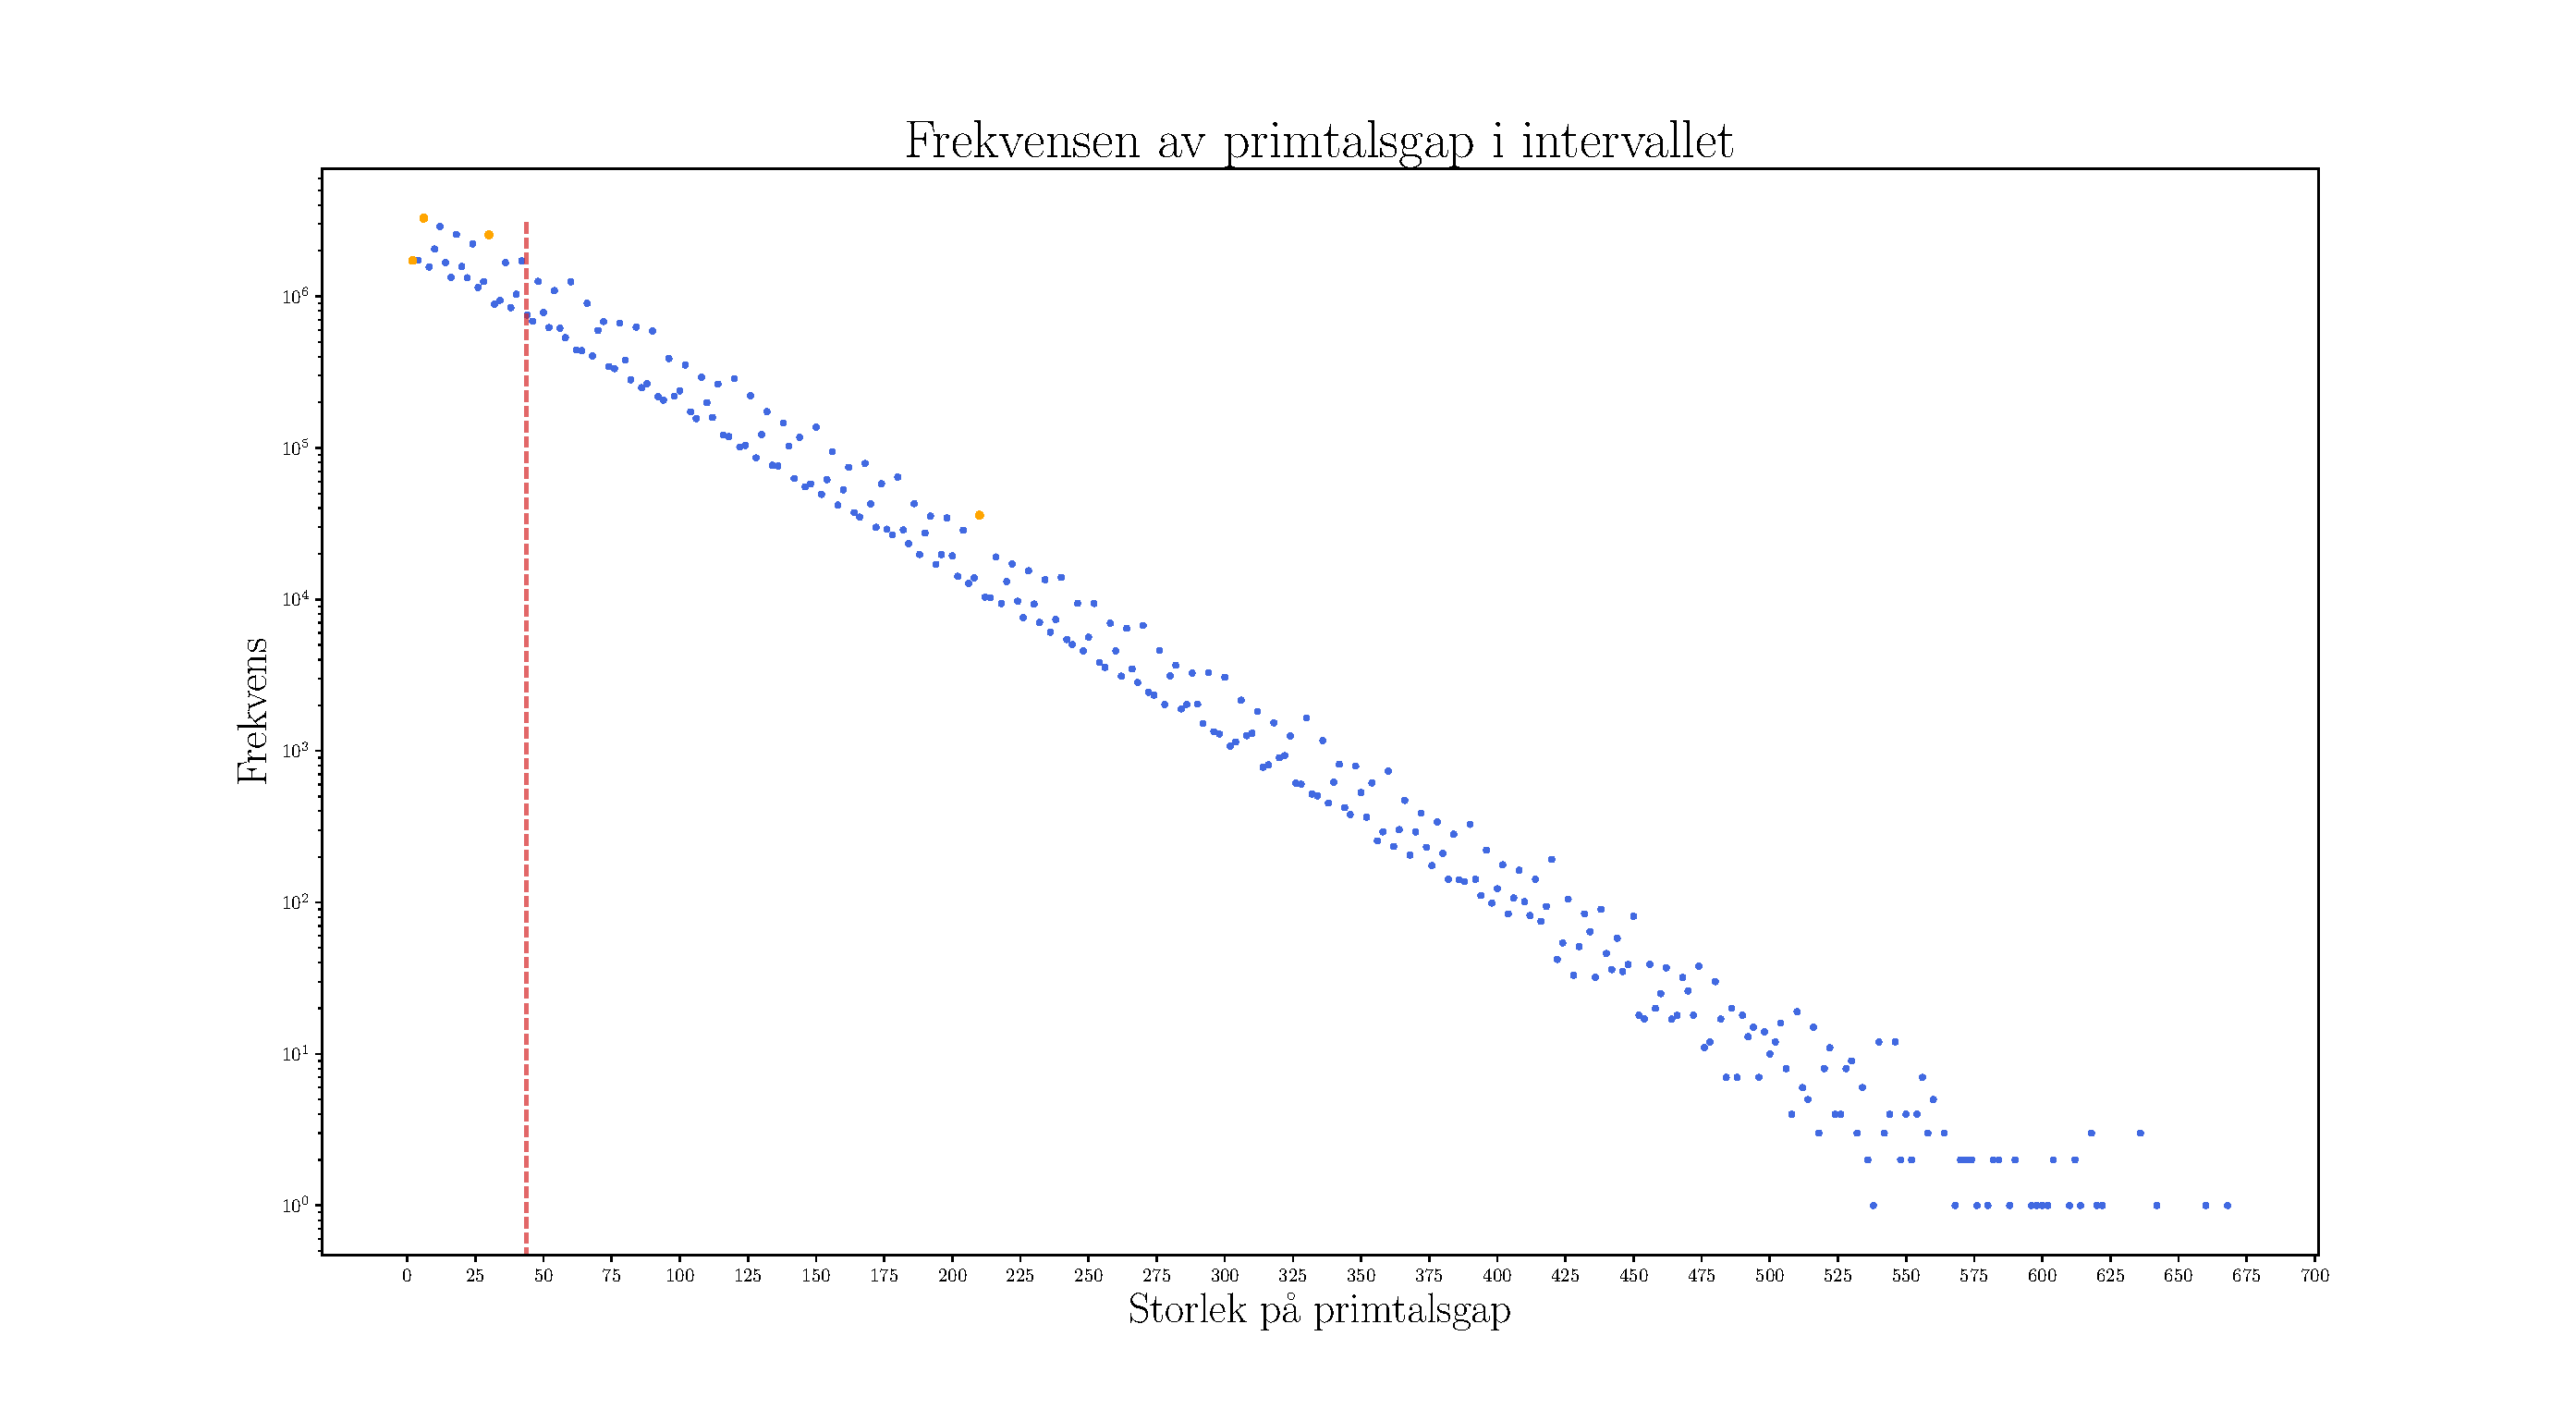
\includegraphics[width = \textwidth]{coen/Images/GapsNoKapps.pdf}
    \caption{I figuren redovisas frekvensen av primtalsgap i intervallet \([n-\Delta,n+\Delta]\), då \(n = 10^{19}\) och \(\Delta = 1.25\cdot10^{9}\). Notera att y-axeln är logaritmerad på grund av den höga frekvensen av små primtalsgap. 
    De orange prickarna anger frekvensen på primtalsgap vars storlek är en primorial (en produkt av de första \textit{n} primtalen).
    Röda linjen markerar den genomsnittliga storleken på primtalsgap i vårt intervall vilket är 43.705.}
    \label{fig:res.gap}
\end{figure}

I figur \ref{fig:res.gap} får vi några insikter kring beteendet av primtalsgap i vårt intervall. 
En kanske överaskande aspekt av grafen är hur rak den är efter logaritmering av y-axeln.
Detta antyder att frekvensen på primtalsgap minskar exponentiellt då dess längd ökar. 
Vi ser att det vanligaste storleken på ett primtalsgap i intervallet är 6 och att det störta gapet är 668.
En detalj som är svår att utläsa från figuren är att det för varje jämnt tal upp till och inklusive 560, finns ett primtalsgap i intervallet med denna storlek.
Enligt primtalssatsen är den förväntade storleken på ett primtalsgap i intervallet ungefär 43.7491, och om vi beräknar den genomsnittliga storleken på primtalsgap i vårt intervall så får vi det till 43.7505.
Återigen stödjer detta resultat legitimiteten av vår kod eftersom datan reflekterar vad som har bevisats i primtalssatsen.

Om vi återgår till primtalstvillingar så säger figuren även något om dem. 
Dessa representeras av primtalsgap med storlek 2, vilket är det sjunde vanligaste primtalsgapet och utgör 3 procent av alla gap i intervallet.

Till sist ger figur \ref{fig:res.gap} intuition för en sats som omnämndes kortfattat i inledningden och säger att det finns oändligt många par av primtal med maximalt 600 steg emellan sig. 
Detta betyder attdet även för stora primtal finns så finns det relativt små primtalsgap.
I vårt intervall är nästan alla primtalsgap mindre än 600, trots att talen i intervallet är stora.
Satsen bevisades med hjälp av nya sållmetoder, specifikt Goldston-Pintz-Yıldırım-metoder utvecklades som år 2005 \cite{GPY}.
I Maynards artikel används vikter liknande de som finns i Selbergs såll, fast på en ännu mer allmän form. 
Sedan 2005 så har 600 steg reducerades ned till 246. 
Ett mål med att fortsätta minska längden är att en dag reducera det till 2 och därmed bevisa primtalstvillingshypotesen.

Såsom mycket annat angående primtal, finns det även en förmodan kopplad till dessa frekvenser ovan och vilket primtalsgap som är mest frekvent upp till en given gräns. 
Som vi ser i figur \ref{fig:res.gap} är 6 (den andra orange pricken) den mest frekventa storleken på primtalsgap i vårt intervall, och speciellt med talet 6 är att det är produkten av de första två primtalen. 
Vi ser också att 30 (den tredje orange pricken) vilket är produkten av de första 3 primtalen, hoppar upp lite från översta delen av bandet, och på samma vis är 210 (den fjärde orange pricken) nästa tal med detta beteende. Förmodan är då att varje \textit{primorial}, produkten av de första \textit{m} primtalen, någon gång blir "hoppmästare".
Förmodan har undersökts direkt med hjälp av numeriska uppskattningsmetoder \cite{primeGaps} som har lyckats visa att 6 är hoppmästaren fram till \(\approx 1.74\cdot10^{35}\) och att 30 sedan tar över titeln fram till \(\approx 10^{425}\).

%Nutidens forskningen kring primtalsgap representerar kulmen på sållteorins teoretisk tillämpning.
%Teorin har utvecklats markant under de senaste hundra åren och tillämpats framgångsrikt på många problem inom talteori.
%Om teorins utveckling fortsätter på denna bana, så kommer fler och fler problem kunna lösas med hjälp av bättre och bättre sållteori.
